\documentclass[10pt, landscape]{article}
\usepackage[scaled=0.92]{helvet}
\usepackage{calc}
\usepackage{graphicx}
\usepackage{multicol}
\usepackage{ifthen}
\usepackage[a4paper,margin=3mm,landscape]{geometry}
\usepackage{amsmath,amsthm,amsfonts,amssymb}
\usepackage{color,graphicx,overpic}
\usepackage{hyperref}
\usepackage{newtxtext} 
\usepackage{enumitem}
\usepackage{graphicx}
\usepackage[table]{xcolor}
\usepackage{mathtools}
\usepackage[document]{ragged2e}
\usepackage{listings}
\setlist{nosep}
\usepackage{subfig}


% for including images
\graphicspath{ {./images/} }


\pdfinfo{
  /Title (ST2334.pdf)
  /Creator (TeX)
  /Producer (pdfTeX 1.40.0)
  /Author (Pei Cheng Yi)
  /Subject (ST2334)
  /Keywords (ST2334, nus,cheatsheet,pdf)}

% Turn off header and footer
\pagestyle{empty}

\newenvironment{tightcenter}{%
  \setlength\topsep{0pt}
  \setlength\parskip{0pt}
  \begin{center}
}{%
  \end{center}
}

% redefine section commands to use less space
\makeatletter
\renewcommand{\section}{\@startsection{section}{1}{0mm}%
                                {-1ex plus -.5ex minus -.2ex}%
                                {0.5ex plus .2ex}%x
                                {\normalfont\large\bfseries}}
\renewcommand{\subsection}{\@startsection{subsection}{2}{0mm}%
                                {-1explus -.5ex minus -.2ex}%
                                {0.5ex plus .2ex}%
                                {\normalfont\normalsize\bfseries}}
\renewcommand{\subsubsection}{\@startsection{subsubsection}{3}{0mm}%
                                {-1ex plus -.5ex minus -.2ex}%
                                {1ex plus .2ex}%
                                {\normalfont\small\bfseries}}%
\renewcommand{\familydefault}{\sfdefault}
\renewcommand\rmdefault{\sfdefault}
%  makes nested numbering (e.g. 1.1.1, 1.1.2, etc)
\renewcommand{\labelenumii}{\theenumii}
\renewcommand{\theenumii}{\theenumi.\arabic{enumii}.}
\renewcommand\labelitemii{•}
\renewcommand\labelitemiii{•}
%  convenient absolute value symbol
\newcommand{\abs}[1]{\vert #1 \vert}
%  convenient floor and ceiling
\newcommand{\floor}[1]{\lfloor #1 \rfloor}
\newcommand{\ceil}[1]{\lceil #1 \rceil}
%  convenient modulo
\newcommand{\Mod}[1]{\ \mathrm{mod}\ #1}
%  for logical not operator, iff symbol, convenient "if/then"
\renewcommand{\lnot}{\mathord{\sim}}
\let\then\Rightarrow
\let\Then\Rightarrow
%  vectors
\newcommand{\vv}[1]{\boldsymbol{#1}}
\newcommand{\VV}[1]{\overrightarrow{#1}}
%  column vector
\newcommand{\cvv}[1]{\left(\begin{smallmatrix}#1\end{smallmatrix}\right)}
\newcommand{\code}[1]{\textcolor{myblue}{\texttt{#1}}}
\newcommand\bggreen{\cellcolor{green!10}}

\makeatother
\definecolor{myblue}{cmyk}{1,.72,0,.38}
\everymath\expandafter{\the\everymath \color{myblue}}
% Define BibTeX command
\def\BibTeX{{\rm B\kern-.05em{\sc i\kern-.025em b}\kern-.08em
    T\kern-.1667em\lower.7ex\hbox{E}\kern-.125emX}}

% Don't print section numbers
\setcounter{secnumdepth}{0}

\setlength{\parindent}{0pt}
\setlength{\parskip}{0pt plus 0.5ex}
%% this changes all items (enumerate and itemize)
\setlength{\leftmargini}{0.5cm}
\setlength{\leftmarginii}{0.4cm}
\setlength{\leftmarginiii}{0.5cm}
\setlist[enumerate,1]{leftmargin=2mm,labelindent=1mm,labelsep=1mm}
\setlist[itemize,1]{leftmargin=2mm,labelindent=1mm,labelsep=1mm}
\setlist[itemize,2]{leftmargin=3mm,labelindent=1mm,labelsep=1mm}
\setlist[itemize,3]{leftmargin=3mm,labelindent=1mm,labelsep=1mm}

%My Environments
\newtheorem{example}[section]{Example}
% -----------------------------------------------------------------------

\begin{document}
\raggedright
\footnotesize
\begin{multicols}{4}


% multicol parameters
% These lengths are set only within the two main columns
\setlength{\columnseprule}{0.25pt}
\setlength{\premulticols}{1pt}
\setlength{\postmulticols}{1pt}
\setlength{\multicolsep}{1pt}
\setlength{\columnsep}{2pt}

\begin{center}
    \fbox{%
        \parbox{0.8\linewidth}{\centering \textcolor{black}{
            {\Large\textbf{ST233}}
            \\ \normalsize{AY22/23 Sem 2}}
            \\ {\footnotesize \textcolor{myblue}{github.com/SeekSaveServe}}
        }%
    }
\end{center}

\subsection{Chapter 1: Basic Concepts of Probability}
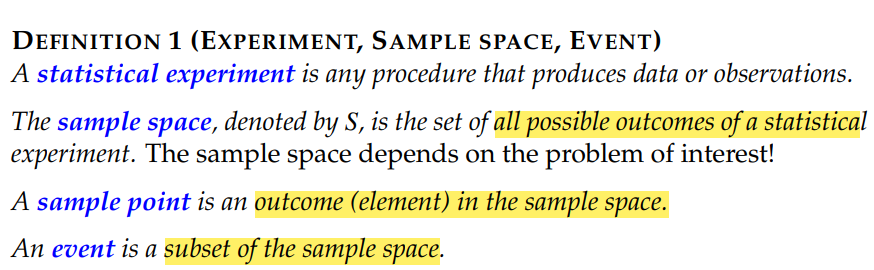
\includegraphics[width=7cm, height=3cm]{images/def1.png}

\textbf{Union:} $A \cup B={x:x\in A \lor x\in B}$ \newline
\textbf{Union of n events:} $\cup^n_{i=1}={x:x\in A_1 \lor x\in A_2...}$ \newline
\textbf{Union:} $A \cap B={x:x\in A \land x\in B}$ \newline
\textbf{Interection of n events:} $\cap^n_{i=1}={x:x\in A_1 \land x\in A_2...}$ \newline
\textbf{Complement:} $A'=x:x\in S \land x \notin A$ \newline
\textbf{Mutually Exclusive:} $A \cap B = \emptyset$ \newline
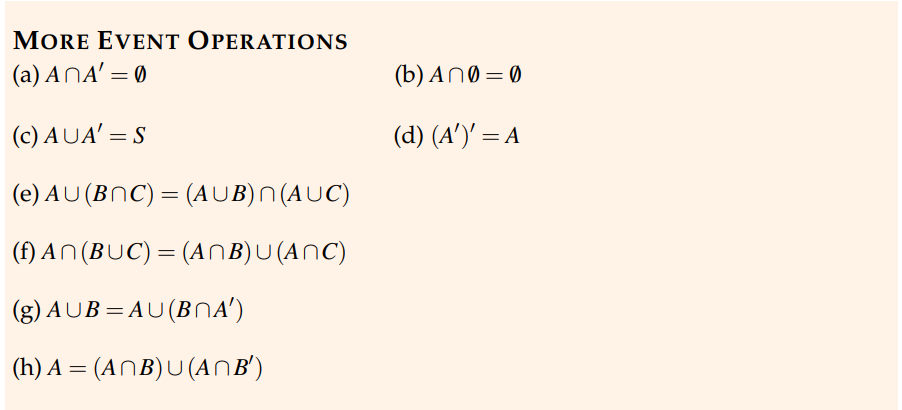
\includegraphics[width=7cm, height=3cm]{operations.png}
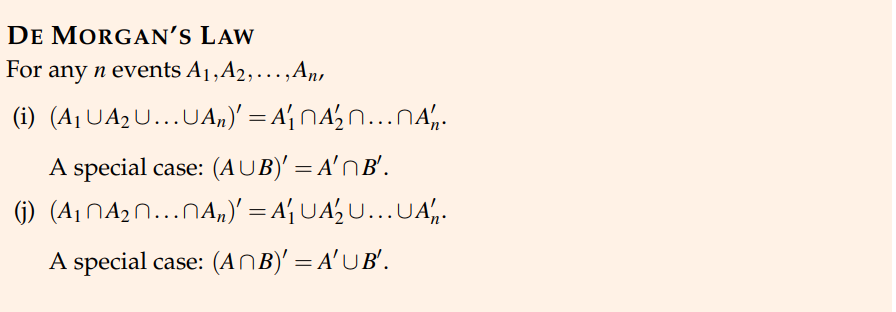
\includegraphics[width=7cm, height=2.6cm]{demorgan.png}

\begin{multicols*}{2}
  \begin{itemize}

    \item[] \textbf{Multiplication}
    \begin{itemize}
      \item[] Sequential experiments
      \item[] $n_1*n_2*...*n_r$ outcomes
    \end{itemize}
    \item[] 
    \item[] \textbf{Addition}
    \begin{itemize}
      \item[] Independent experiments
      \item[] $n_1+n_2+...+n_r$ outcomess
    \end{itemize}
  \end{itemize}
\end{multicols*}

\textbf{Permutation:} $P^n_r=\frac{n!}{(n-r)!}=n(n-1)...(n-(r-1))$\newline
Selection and arrangement of r objects out of n. Order is considered. \newline

\textbf{Combination:} $C^n_r=\frac{n!}{r!(n-r)!}=\frac{n(n-1)...(n-(r-1))}{r!}$\newline
Selection of r objects out of n. Order is not considered. $C^n_r=C^n_{n-r}$\newline

\textbf{Axioms and Properties of Probability}
\begin{itemize}
  \item[1] $0\leq P(A)\leq 1$
  \item[2] P(S)=1
  \item[3] $P(A\cup B)=P(A)+P(B)$ if A and B are \textbf{mutex} (not to be confused with independence)
  \item[4] P($\emptyset$)=0
  \item[5] P($A_1 \cup A_2 \cup...A_n$)=$\sum_{i=1}^{n}A_i$ 
  \item[6] P($A'$)=$1-P(A)$
  \item[7] $P(A\cup B)=P(A)+P(B)-P(AB)$
  \item[8] P(A)=$P(A\cap B) + P(A\cap B')$   
  \item[9] $A \subset B \rightarrow P(A) \leq P(B)$
  \item[10] $P(A_1)=P(A_2)=...=P(A_k) \rightarrow for B \subset S, P(B)=\frac{|B|}{|S|}$ 
\end{itemize}

\textbf{Conditional Probability (B occurs given A):} $P(B|A)=\frac{P(A\cap B)}{P(A)}$ \newline
\textbf{Multiplication rules} \newline
 $P(A\cap B)=P(A)P(B|A)$ if $P(A)!=0$ \newline
$P(A\cap B)=P(B)P(A|B)$ if $P(B)!=0$ \newline
\textbf{Inverse Probability Formula:} $P(A|B)=\frac{P(B|A)P(A)}{P(B)}$ \newline
\textbf{Indepenence} $A\bot B iff P(A \cap B)=P(A)P(B)$ This implies $P(A|B)=P(A) \text{ and } P(B|A)=P(B)$ \newline
\textbf{Partition} $A_1,A_2...A_r$ are mutually exclusive and $\sum_{i=1}^{n}A_i=S$ \newline

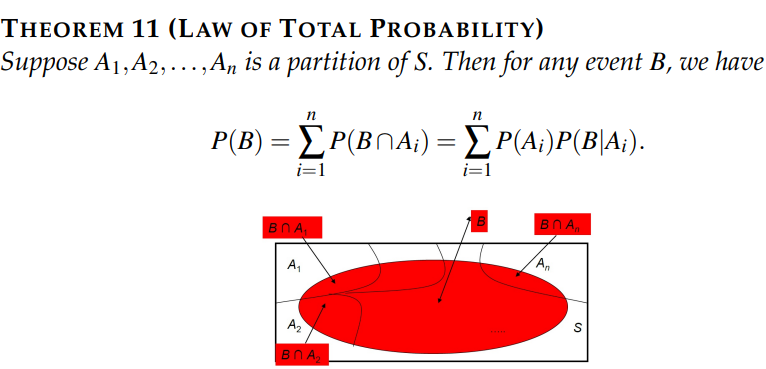
\includegraphics[width=7cm, height=3cm]{lotp.png}
$P(B)=P(A)P(B|A)+P(A')P(B|A')$ \newline

\textbf{Bayes' theorem} $P(A_k|B=\frac{P(B|A)P(A_k)}{P(A)P(B|A)+P(A')P(B|A')})$ \newline
\textbf{Bayes' Theorem (n=2):} $P(A|B)=\frac{P(B|A)P(A)}{\sum_{i=1}^{n}P(A_i)P(B|A_k)}$ Denom is P(B) \newline

\subsection*{L2:Random Variables}
Random variable X is a function from S to $R$ \newline
Uppercase letters denote random variables \newline
Lowercase letters denote observed values of random variables \newline

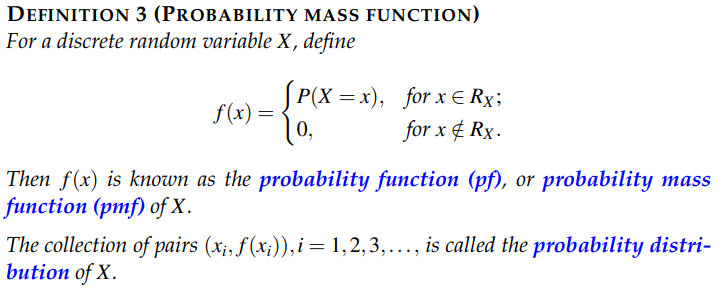
\includegraphics[width=7cm, height=3cm]{pmf.png}
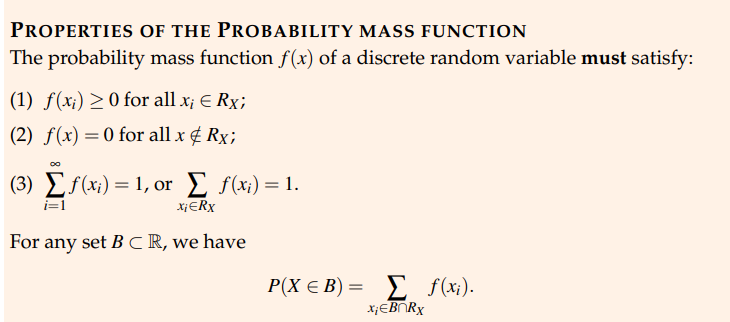
\includegraphics[width=7cm, height=3cm]{pmf_properties.png}
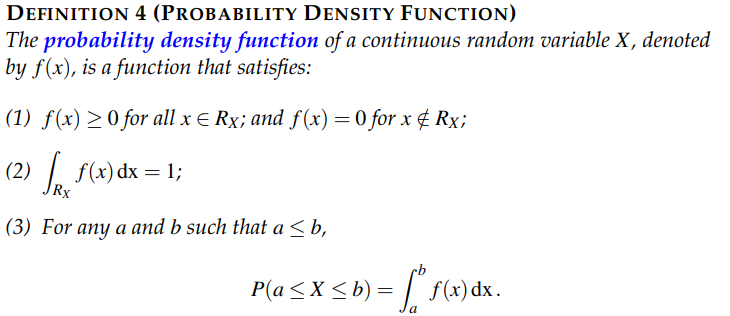
\includegraphics[width=7cm, height=3cm]{pdf.png} \newline
note: $P(a<X<b) = P(a\le X \le B)$ \newline
To check that a function is a PDF, chcek conditions 1 and 2 \newline

\textbf{Cumulative Distribution Function:} $F(x)=P(X\le x)$ and $P(a \le b) = P(X \le b) - P(X \le a) = F(b) - F(a-)$ \newline

\textbf{Deriving CDF from probability distribution} \newline
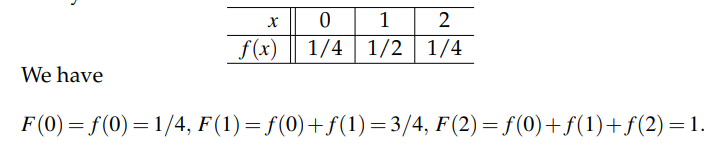
\includegraphics[width=7cm, height=2.3cm]{pf_cdf.png}


\textbf{Deriving probability distribution from cdf} \newline
\begin{multicols*}{2}
  \begin{itemize}
    \item[] 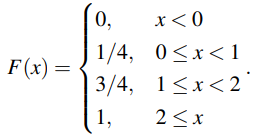
\includegraphics[width=3cm, height=2cm]{cdf_pf.png}
    \begin{itemize}
      \item f(1)=P(X=0)=F(0)-F(0-)=$\frac{1}{4}$-0=$\frac{1}{4}$
      \item f(2)=P(X=1)=F(1)-F(1-)=$\frac{3}{4}$-$\frac{1}{4}$=$\frac{1}{2}$
      \item f(3)=P(X=2)=F(2)-F(2-)=1-$\frac{3}{4}$=$\frac{1}{4}$
    \end{itemize}
  \end{itemize}
\end{multicols*}

\textbf{CDF - Continuous Random Variable} 
\begin{itemize}
  \item F(X) assumes different values in $R_x$ when F(X)!=0 
  \item F(X) is always non-decreasing (for discrete varaible too) $x_1<x_2 \rightarrow F(x_1)<F(x_2)$
  \item Probability function and CDF is one-to-one and uniquely determined
  \item $0<F(x)<1$ 
  \item (discrete), $0<f(x)<1$
  \item (continuous), $f(x) \ge 0$ but $f(x)$ is not necessarily $\le 1$. While the PDF itself cannot exceed 1, there are points within its range that are greater than 1
\end{itemize}
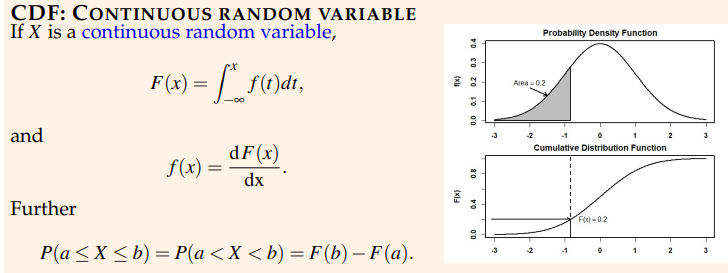
\includegraphics[width=7cm, height=3.5cm]{cdf_random.png}

\textbf{Find CDF of a continuous random variable} \newline
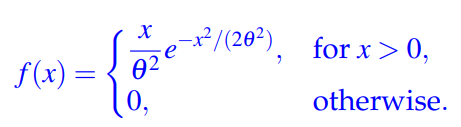
\includegraphics[width=7cm, height=1.5cm]{p2.png}
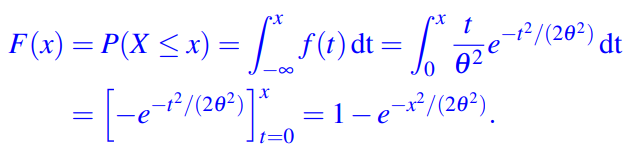
\includegraphics[width=7cm, height=2cm]{p1.png}

\textbf{Discrete: Expectation (mean) and Variance}
\begin{itemize}
  \item $E(X)=\sum_{x \in R_x}x_if(x_i)=\mu_x$
\end{itemize}

\textbf{Random: Expectation (mean) and Variance}
\begin{itemize}
  \item $E(X)=\mu_x=\int_{-\infty}^{\infty}xf(x)dx= \infty_{x \in R_x}xf(x)dx$
  \item The mean of X is not necessarily a possible value
\end{itemize}

\textbf{Properties of Expectation}
\begin{itemize}
  \item[1] $E(aX+b)=aE(x)+b$
  \item[2] $E(X+Y)=E(X)+E(Y)$
  \item[3] (discrete) $E|g(x)|= \sum_{x \in R_x}g(x)f(x)$
  \item[3] (continuous) $E|g(x)|= \int_{x \in R_x}g(x)f(x)dx$
  \item Using properties 1, 2 we have $E(a_1X_1+a_2X_2+...+a_kX+k)=a_1E(X_1)+...+a_kE(X_k)$
\end{itemize}

\textbf{Variance} 
\begin{itemize}
  \item $Var(X)=\sigma_x^2=E(X-\mu_x)^2=E(X^2)-E(X)^2$
  \item (discrete) $Var(X)=\sum_{x \in R_x}(x-\mu_x)^2f(x)$
  \item (continuous) $Var(X)=\int_{-\infty}^{\infty}(x-\mu_x)^2f(x)dx$
  \item V(X) $le$ 0 for any X, V(X)=0 when X is a constant
  \item 
\end{itemize}


\end{multicols}
\end{document}